\chapter{Methodology} \label{cap:methodology}

This chapter will explain the methods used to conduct the present work that aims to compare the performances of the manifold learning methods metric MDS, LLE, and t-SNE. We will start by describing utilized datasets and proceed with the experimental procedure. Finally, we will describe the system specification and tools used to conduct the experiments a give a brief insight into the acquisition of the data resulting from the experiments.

\section{Datasets}

Various datasets from public sources were used to conduct the experiments in this work. The selected datasets contain different types of structures, such as circular-, linear-, or arbitrarily complex- structures. We will be focusing on datasets that have a reasonable amount of instances. It must be large enough to ensure high quality and small enough to ensure that the execution times do not grow in an exponential fashion. Therefore, we chose the 3D-Mammoth, a transformed version of it, and the COIL-20 datasets to evaluate the performance of the different manifold learning methods. In the following, we will introduce the datasets in detail.

\subsection{3D-Mammoth}

The 3D point cloud of a mammoth skeleton is not well known and is only used by a few researchers on the task of manifold learning. This dataset was digitalized by "Smithsonian 3D DIGITALIZATION" $^1$. It originally consisted of 50,000 data points, but we will just use a random sample of 10,000 data points. We will reduce the dataset from 3 to 2 dimensions and not to 1 because we want to have as little information loss as possible. Furthermore, it has no natural cluster structures as the data points are connected throughout to form a mammoth skeleton. Still, the dataset is especially suited for observing the behavior of local or global structure preservation. For visualization purposes, the data points were colored to have a better overview of where body parts appear in the low-dimensional embedding. The colored dataset can be viewed in Figure. \ref{fig:mammoth_original_plot}. \cite{mammoth}
\begin{figure}[!]
	\centering
	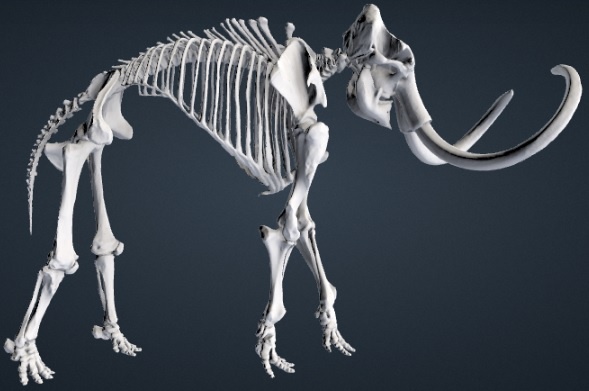
\includegraphics[width=0.9\columnwidth]{images/mammoth-skelleton.jpg}
	\caption[3D Mammoth Skeleton]{Digitalized Mammoth Skeleton, adapted from \footnotemark}
    \label{fig:mammoth-skelleton}
\end{figure}
\footnotetext{\url{https://3d.si.edu/explorer/woolly-mammoth}}

\subsection{Transformed 3D-Mammoth}

The 3D-Mammoth dataset has the special property that it is continuous, meaning that data points have a neighbor that is very close to it. If this applies to every data point it means that the whole dataset/manifold is "connected" (Figure \ref{fig:mammoth_original_plot}). To evaluate the impact of the continuity property of a dataset on dimensionality reduction methods, we decided to transform the original dataset to a similar non-continuous version. Therefore we are interested in the question if there are methods that prefer continuous datasets.
The transformation, which can be seen in Figure \ref{fig:mammoth_trans_plot}, was achieved by first applying the clustering algorithm $k$-Means with such parameter so that the rip cage was 
well clustered and then this cluster was moved by $+50$ on the z-axis. This results in a dataset where the head, the rib cage, the front legs, and the back legs with the tail are not connected anymore. Note that a tiny bit of the end of the tail is also colored blue which is a result of $k$-Means finding convex clusters. Also important to note is that this clustering did not derive as it is. Instead, we combined two clusters to obtain a single cluster for the entire rib cage.
The number of points within a cluster is as follows:

\begin{figure}[!]
     \centering
     \begin{subfigure}[t]{0.45\columnwidth}
    	\centering
    	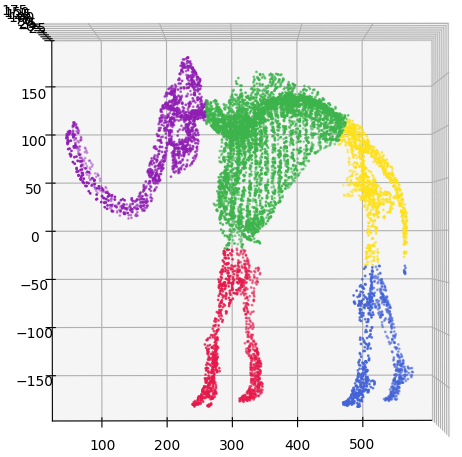
\includegraphics[width=\columnwidth]{images/mammoth_original_plot.png}
    	\caption{Original 3D-Mammoth}
        \label{fig:mammoth_original_plot}
    \end{subfigure}
     \hfill
     \begin{subfigure}[t]{0.45\columnwidth}
    	\centering
    	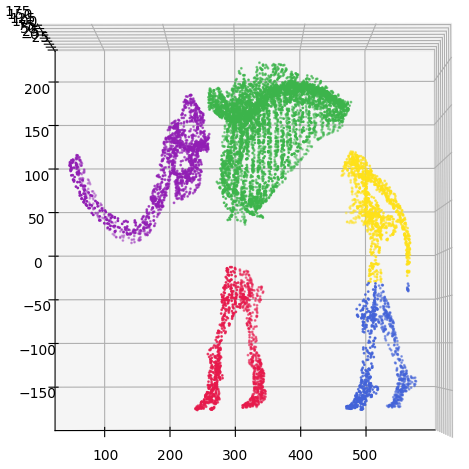
\includegraphics[width=\columnwidth]{images/mammoth_trans_plot.png}
    	\caption{Transformed 3D-Mammoth}
        \label{fig:mammoth_trans_plot}
    \end{subfigure}
     \caption[Original and Transformed Mammoth]{Illustration of how the Mammoth dataset was transformed and how the segments were colored to better evaluate the visualization of the low-dimensional embedding.}
    \label{fig:orig_vs_trans_mammoth}
\end{figure}
\begin{table}[]
\centering
\begin{tabular}{|c|c|c|c|c|}
\hline
{\textcolor{rib_cage}{\textbf{Rib cage}}} &
  {\textcolor{head}{\textbf{Head}}} &
  {\textcolor{back_tail}{\textbf{Back \& Tail}}} &
  {\textcolor{front_feet}{\textbf{Front feet}}} &
  {\textcolor{back_feet}{\textbf{Back feet}}} \\ \hline
5199 &
  1608 &
  1173 &
  1148 &
  872 \\ \hline
\end{tabular}
\caption[Number of Points in 3D-Mammoth]{Coherent regions/structures of 3D-Mammoth with their number of points in descending order.}
\label{tab:num_datapoints_mammoth}
\end{table}

\subsection{COIL-20}

This dataset was proposed by Columbia University in 1996 and stands for Columbia Object Image Library-20. It contains size-normalized, gray-scale images of 20 different objects with different shapes and characteristics, and therefore it has a ground truth clustering. The collection of all images can be seen in Figure \ref{fig:coil-20}. For every object, 72 images were taken in equally spaced orientations of 5° (Figure \ref{fig:coil-20_duck}), resulting in a total of 1440 images in a 128x128 pixel format. This dataset is well known in the research community but not as widely used as, for example, MNIST or the Iris flower dataset. The dimensionality of the original space is 16384. The dimensionality of the embedded space will be 3 and not lower because we want to reduce the dataset so that we can visualize it and have as little information loss as possible. \cite{COIL-20}
\begin{figure}[!]
	\centering
	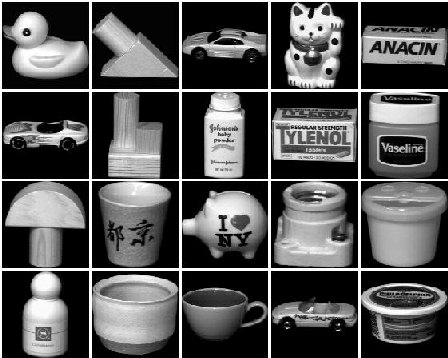
\includegraphics[width=0.9\columnwidth]{images/coil-20.jpg}
	\caption[COIL-20 Images]{COIL-20 image collection, adapted from \cite{COIL-20}}
    \label{fig:coil-20}
\end{figure}
\begin{figure}[!]
	\centering
	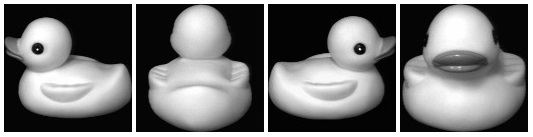
\includegraphics[width=0.9\columnwidth]{images/coil-20_duck.jpg}
	\caption[COIL-20 Duck Images]{Rubber Duck from COIL-20 dataset in different angles, adapted from \cite{COIL-20}}
    \label{fig:coil-20_duck}
\end{figure}

\section{Experimental Procedure} \label{sec:exp.prod}

In this section, we want to introduce the experimental procedure we conceptualized for our work. We will investigate the behaviors of the manifold learning methods MDS, LLE, and t-SNE for all experiments. The variety of these methods is representative of manifold learning because they have different focuses of information preservation, namely distance-, neighborhood- and probability distribution- preservation. In the following, we will describe the experiments we want to conduct in detail. Also, we will go into detail about why we chose specific aspects, see them as relevant, and how we want to achieve the quality evaluation of the different method results. At last, we will bring all the experiments together into one whole experiment procedure. For this purpose, we constructed a pipeline.

\subsection{Preservation of Distances} \label{subsec:dist}

To evaluate the performance of manifold learning methods, one can evaluate the preservation of global structures like the overall shape of the dataset. This can be done by calculating the pairwise distances of all points in high and low dimensional space, resulting in \textit{distance matrices} $\Delta^D$ and $\Delta^d$ respectively. A general $n \times n$ distance matrix is defined as
\begin{equation}
    \Delta=
    \begin{bmatrix}
        0 & d_{12} & d_{13} & \cdots & d_{1n}\\
        d_{21} & 0 & d_{23} & \cdots & d_{2n}\\
        d_{31} & d_{32} & 0 & \cdots & d_{3n}\\
        \vdots & \vdots & \vdots & \ddots & \vdots\\
        d_{n1} & d_{n2} & d_{n3} & \cdots & 0
    \end{bmatrix}
\end{equation}
where $n$ is the number of data points, and $d$ is a distance metric. In our case, it will be Euclidean. This matrix has the property $d_{ii}=0$ because the distance from one point to itself is nonexistent, reflecting the reflexivity property of our metric. Another property is that the matrix is symmetric, meaning $d_{ij}=d_{ji}$, because the distance from one point to another is the same as the distance from the other point to the one. After calculating the distance matrices, these have to be normalized by dividing all values by the maximal value.
\begin{equation}
    \forall i,j: d_{ij} = \frac{d_{ij}}{\max_{i,j} (d_{ij})}
\end{equation}
This serves the purpose of yielding values between 0 and 1 because we are interested in the distance preservation ratio instead of real distances. This decision is based on one phenomenon regarding the distances of data points in high dimensional space, namely that they exhibit very high values compared to data points in low dimensional space, which was already addressed in Subsection \ref{subsubsec:crowding}. Thus relying on real distances would result in very high differences between high- and low-dimensional distance matrices. Thereafter both matrices $\Delta^D$ and $\Delta^d$ are subtracted from each other to yield the distance difference ratios of the high and low dimensional data points.
\begin{equation}
    \Delta^D - \Delta^d = [d_{ij}^D] - [d_{ij}^d] = [d_{ij}^D - d_{ij}^d] = [d_{ij}^{Dd}] = \Delta^{Dd}
\end{equation}
At last, every entry is folded into one value, enabling us to compare the manifold learning methods. This procedure of folding is achieved by computing the \textit{Frobenius norm}
\begin{equation}
    ||\Delta^{Dd}||_F = \sqrt{\sum_{i,j} (d_{ij}^{Dd})^2}.
\end{equation}
A low Frobenius norm would indicate that most of the distances $\Delta^d$ are similar to those of $\Delta^D$. Hence we have an indication that the pairwise distances are (mostly) well preserved. While a high Frobenius norm indicates, on the contrary, bad preservation of distances. Note that the range of possible values for the norm is dataset-specific and depends on the number of data points. The more the number of data points the more pairwise distances exist and therefore there are more values that are being folded together. [\cite{wiki_dist_matrix}, \cite{wiki_matrix_norm}]

\subsection{Preservation of Neighborhoods} \label{subsec:kNN}

To evaluate the performance of manifold learning methods, one can also evaluate the preservation of local structures like neighborhoods. In general, if two points in the original space are close to each other, they are considered similar. Therefore they should be embedded in low dimensional space while preserving the closeness. Nonetheless, in the special case of datasets being susceptible to short-circuiting (e.g., in Subsection \ref{subsubsec:short}), this does not always hold and depends strongly on the magnitude of the local neighborhood. For this purpose, using the \textit{trustworthiness} measure to evaluate the local structure preservation has prevailed and is therefore popular among the related literature. This measure has values ranging from 0 to 1, while a higher value indicates better preservation. Therefore, an embedding is considered entirely trustworthy if the $k$-nearest-neighbors ($k$NN) in the original space are also $k$NN in the embedded space. Informally the authors define the measure as: "Trustworthiness of the neighborhoods is quantified by measuring how far from the original neighborhood the new data points entering a neighborhood come" \cite{trustworthiness}. The formal definition is
\begin{equation}
    T(k)=1-\frac{2}{nk(2n-3k-1)}\sum^n_{i=1}\sum_{j\in\mathcal{N}^k(y_i)}\max(0,(r(\mathcal{N}^k(x_i),x_j)-k))
\end{equation}
where $n$ is the number of data samples, $r(\mathcal{N}^k(x_i),x_j)$ denotes the rank of point $x_j$ in the $k$-neighborhood of $x_i$ in the original space and $\mathcal{N}^k(y_i)$ indicates the set of neighbors of $y_i$ in the embedded space. [\cite{trustworthiness}, \cite{Gisbrecht15}]

\subsection{Clusterability on Embeddings} \label{subsec:cluster}

One can also use clustering algorithms to analyze the performance of manifold learning methods. Therefore three different cases must be distinguished. The first case emerges if the clustering in high dimensional space remains the same in low dimensional space. One can state that the manifold learning method used to yield the low dimensional embedding performed well in structure preserving. The second case emerges if the clustering in the embedded space is worse than the one in the original space, then the cluster structures could not be preserved. The third case emerges if the clustering somehow got better considering the compactness and separability of the clusters. This fact can only be captured by internal measures, which we will discuss in the following. In the case where the clustering could not be preserved, it may also mean that the clustering algorithm used for this task is unsuitable for the specific dataset. Because of this limitation, we use multiple clustering algorithms with different focuses on finding cluster structures to enable the making of a better statement about the manifold learning methods instead of the clustering methods. Therefore we will use the methods $k$-Means and DBSCAN introduced in Section \ref{sec:clustering}. We will employ these methods on the high dimensional 3D-Mammoth and the low dimensional COIL-20 and 3D-Mammoth datasets. For the high dimensional COIL-20 dataset, there is already a clustering existing. There are different evaluation measures with different types to evaluate the resulting clustering. Those types are \textit{internal} and \textit{external} measures. \cite{Gisbrecht15}

Former is a measure that does not evaluate the clustering with the help of the ground truth; instead, it just gives insight into how well the clusters are, meaning how well the clusters are separated and how dense they are. In our case, we will use the \textit{silhouette coefficient/score} (SC). The value of this score ranges from $-1$ to $1$. The higher the score, the denser and better separated the clusters are, and the lower the value the opposite holds. Values near $0$ indicate overlapping clusters. The definition of this coefficient on a single point is:
\begin{equation}
    s(i)=\frac{b(i)-a(i)}{\max \{ a(i),b(i) \} }
\end{equation}
where $i$ is a point either in the original space or embedded space $i\in \{ x_i,y_i \}$. To further understand this definition, we need the notion of a \textit{clustering} $\mathcal{C}$ with \textit{clusters} $C_I, C_J \in \mathcal{C}$, where $I, J \in \{0,..,k\}$. Note that $|\mathcal{C}| = k$, while $k$ is the number of clusters, for example, defined in $k$-Means. As point $i$ can be high and low dimensional space, the clustering $\mathcal{C}$ can also be $\mathcal{C}^D$ or $\mathcal{C}^d$, which are just special cases.
\begin{equation}
    a(i)= \frac{1}{|C_I|} \sum_{j\in C_I} d_{ij}
\end{equation}
is one formula that we need to calculate the silhouette score. It calculates the average distances from point $i$ all point other points $j$ within a cluster.
\begin{equation}
    b(i)= \min_{C_J \in \mathcal{C}, C_J\neq C_I} (\frac{1}{|C_J|}\sum_{j\in C_J}d_{ij})
\end{equation}
is the other formula that we need that calculates the average distance from point $i$ to points $j$ of the nearest cluster. An illustration of the calculation of the silhouette coefficient can be seen in Figure \ref{fig:silhouette}. Note that $s(i)$ calculates the silhouette score for a single point. We will calculate the mean scores for all points to yield a single value to enable easier comparisons. Important to note is that this evaluation measure highly favors methods that result in convex-shaped clusters like $k$-Means. However, this should not deter us as we are interested in evaluating the manifold learning methods. We will be analyzing the performances of manifold learning methods with a combined view of the clustering algorithms. [\cite{silhouette}, \cite{sklearn_silhouette}]
\begin{figure}[!]
	\centering
	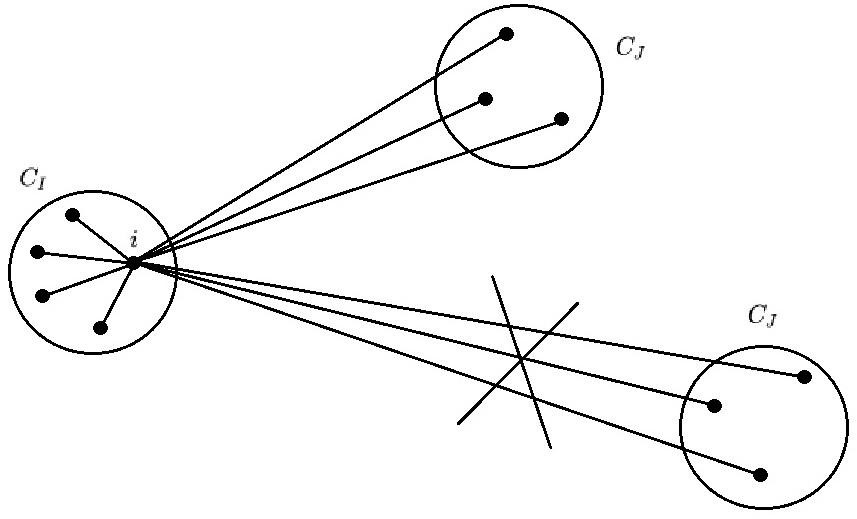
\includegraphics[width=0.9\columnwidth]{images/silhouette.jpg}
	\caption[Silhouette Coefficient]{Illustration of the calculation of the silhouette coefficient, adapted from \cite{silhouette}}
    \label{fig:silhouette}
\end{figure}

Latter, meaning the external measure, is a measure that makes use of ground truth clustering. Therefore the advantage over internal measures is that these do not make any assumption about the cluster shapes or any other model-specific assumptions like density and variance. One external measure we will be using in this work is the \textit{adjusted rand index} (ARI). This is a special form of the \textit{rand index}, which is defined as
\begin{equation}
    RI = \frac{TP+TN}{TP+TN+FN+FP}.
\end{equation}
This formula divides the number of all truly clustered pairs of points by all possible pairs of points. To elaborate on this definition, we need to know the ground truth clustering $\mathcal{C}^D$ in the original space and the calculated clustering $\mathcal{C}^d$ in the embedded low dimensional space. We also need to know that $C^D_I, C^D_J \subseteq \mathcal{C}^D$ and $C^d_K, C^d_L \subseteq \mathcal{C}^d$ are clusters where $I,J,K,L \in \{0,..,k\}$ and $I\neq J, K\neq L$. With this prior knowledge, we can define all needed expressions for the $RI$ formula.
\begin{equation}
    TP = |\{(i,j) : i,j \in C^D_I, i,j \in C^d_K \}|
\end{equation}
\begin{equation}
    TN = |\{(i,j) : i \in C^D_I, j \in C^D_J, i \in C^d_K, j \in C^d_L \}|
\end{equation}
\begin{equation}
    FN = |\{(i,j) : i,j \in C^D_I, i \in C^d_K, j \in C^d_L \}|
\end{equation}
\begin{equation}
    FP = |\{(i,j) : i \in C^D_I, j \in C^D_J, i,j \in C^d_K \}|
\end{equation}
$TP$ stands for true positive, $TN$ for true negative, $FN$ for false negative and $FP$ for false positive. This version can be updated to the corrected-for-chance version (adjusted). The formula is then extended by the expected value of the rand index, indicating the result of random clustering, and then divided by the maximal possible value.
\begin{equation}
    ARI=\frac{RI-\mathbb{E}[RI]}{\max(RI)-\mathbb{E}[RI]}
\end{equation}
The result of this formula can then range from $-1$, indicating clustering that was mostly false classified, to $1$, indicating mostly true classified pairs of points. Values near $0$ indicate a random clustering result. [\cite{rand_index}, \cite{sklearn_clu_eval}, \cite{wiki_rand_index}]

Another external evaluation measure is the \textit{adjusted mutual information} (AMI) which is defined as 
\begin{equation}
    AMI(\mathcal{C}^D,\mathcal{C}^d)= \frac{MI(\mathcal{C}^D,\mathcal{C}^d) - \mathbb{E}(MI(\mathcal{C}^D,\mathcal{C}^d))}{\max(H(\mathcal{C}^D), H(\mathcal{C}^d)) - \mathbb{E}(MI(\mathcal{C}^D,\mathcal{C}^d))}.
\end{equation}
This measure is similar to ARI in that it calculates the similarity between clusterings. More precisely, it quantifies the information shared by these. It is also a corrected-for-chance version (adjusted) of the \textit{mutual information} (MI) measure which is defined as:
\begin{equation}
    MI(\mathcal{C}^D,\mathcal{C}^d)=\sum^{|\mathcal{C}^D|}_{I=1} \sum^{|\mathcal{C}^d|}_{K=1} P_{\mathcal{C}^D\mathcal{C}^d}(I,K) \log \frac{P_{\mathcal{C}^D\mathcal{C}^d}(I,K)}{P_{\mathcal{C}^D}(I)P_{\mathcal{C}^d}(K)}
\end{equation}
where 
\begin{equation}
    P_{\mathcal{C}}(I) = \frac{|\mathcal{C}_I|}{N}
\end{equation}
is the probability that some random point belongs to one cluster and 
\begin{equation}
    P_{\mathcal{C}^D\mathcal{C}^d}(I,K) = \frac{|\mathcal{C}^D_I \cap \mathcal{C}^d_K|}{N}
\end{equation}
is the probability that some random point belongs to both clusters.
The used entropy for AMI is:
\begin{equation}
    H(\mathcal{C}) = - \sum^{|\mathcal{C}|}_{I=1} P_{\mathcal{C}}(I) \log P_{\mathcal{C}}(I).
\end{equation}
Note that the value range is exactly as in ARI. \cite{wiki_mutual_info}

\subsection{Robustness w.r.t. Parameters}

As we have already mentioned in the Subsection \ref{subsubsec:parameter_tuning} that the parameter tuning of the manifold learning methods is crucial because it can dramatically impact the quality of the outcome. It relies on the dataset and its properties. In some cases, it may have almost no severe effect if the parameter values are changed, and in other cases, it may have a heavy impact. Therefore we will determine which parameter or parameter ranges are best suited for a specific dataset and evaluation measure. The datasets that we will be investigating are the COIL-20 and 3D-Mammoth datasets. 

On those datasets, we will deploy the manifold learning methods MDS, LLE, and t-SNE. For MDS, there is no need for parameter tuning as it does not depend on a parameter, unlike in LLE and t-SNE, where we will tune the neighborhood size $k$ for LLE and the $perplexity$ for t-SNE. For the initial parameter range, we will use the maximal possible range from $1$ to $n$, where $n$ denotes the number of instances. As there are a lot of instances in the datasets, we will choose a higher step size, depending on the computation time. This yields the purpose of finding all relevant parameter settings. If there are small areas where a lot of variation in the values happens, there is the possibility to "zoom" in a specific range, resulting in a lower step size. There are two criteria that we will be optimizing while tuning the parameters. One criterion will be the distance preservation capability with the Frobenius norm of the delta distance matrices that we introduced in Subsection \ref{subsec:dist} and the neighborhood preservation capability with the trustworthiness measure that we introduced in Subsection \ref{subsec:kNN}.

Furthermore, we will be evaluating the clusterability of the manifold learning methods by deploying the clustering algorithms $k$-Means and DBSCAN. These also have parameters that must be set, raising the need for tuning them as well as finding the optimal settings. For $k$-Means, it will be the number of clusters $k$, which will tune by starting with $2$ and successively raising k until convergence. For DBSCAN we will be tuning the parameter $Eps$ in the range of $[mindist:maxdist]$ where $mindist$ is the minimal distance between two points and $maxdist$ is the maximal pairwise distance in the dataset. $MinPts$ is the second parameter, which we will tune in the range of [1:n], similar to the parameter tuning for the manifold learning methods above. The step sizes are again dependent on the computation times. The measures we will use to evaluate the clusterability are SC, ARI, and AMI, as we have introduced in the Subsection \ref{subsec:cluster}.

\subsection{Visualization Quality} \label{subsec:vis_qual}

In this work, we will mainly focus on objective evaluation measures, as you have seen in the previous sections because it leads to no in-depth insight since it is highly subjective. Nevertheless, we will look into the visualization and do a visual examination to answer whether a good objective measure also implies a good visualization. For this examination, we will be as objective as possible and evaluate the visualization concerning the preservation of coherent regions, unique characteristics, and shapes.
We will construct a heatmap after calculating the delta pairwise distance matrix. With this type of visualization, we can see at a glance which regions have been well preserved. In the case of the 3D-Mammoth datasets, we will go a little bit further and calculate the mean of all pairwise distances from a single to all other datapoints. This is done to quantify the distance preservence of datapoints. After that, we will color the points that could not be preserved well red and the points that could be preserved yellow/white in the high dimensional 3D-Mammoth. This allows us to see which areas/structures the manifold learning methods preserved poorly. \cite{Gisbrecht15}

\subsection{Merging it together} \label{subsec:merging}

This subsection merges the previously introduced experiments into one monolithic experiment. Therefore we designed a pipeline which can be seen in Figure \ref{fig:pipeline}. This pipeline gets a configuration $Conf$ as input which consists of four parameters: dataset $DS$, dimensionality reduction method $DR$, evaluation criterion $EC$, and clustering algorithm $CLU$. These parameters are elements of sets that are defined in the Figure. Since $|DS|=2$, $|DR|=3$, $|EC|=2$ and $|CLU|=2$ we get a total of $2 \cdot 3 \cdot 2 \cdot 2=24$ different configurations that can serve as inputs.
On the top of the pipeline is $DS^D$ indicating the high dimensional dataset. This dataset is then reduced by a dimensionality reduction method $DR$. This yields low dimensional embeddings of the initial datasets $DS_1^d, .., DS_n^d$ while $n$ is the number of parameter settings. With these $n$ embeddings, we chose an evaluation criterion, for example, distance preservation. These results are then evaluated and compared to the high dimensional evaluation criterion $EC^D$. In this example, $EC^d$ could be a distance matrix computed from a low dimensional embedding and $EC^D$ a distance matrix computed from the corresponding high dimensional dataset. In the next step, just the best parameter which yielded the best result w.r.t the evaluation criterion is extracted and further used to deploy a clustering algorithm on the low dimensional clustering $CLU^d$, which is then compared to the clustering of the high dimensional dataset $CLU^D$. Using just the best parameter of the distance- and neighborhood-preservation for the clustering algorithm is done to overcome the issue of parameter tuning too much, namely to prevent a combination of parameters from manifold learning and clustering that would be computationally prohibitive. The advantage of this approach is that it enables us to see if the parameters that best preserved the global or local structures also yield good clustering results or if the parameter should be tuned independently for the clustering task.

\begin{figure}[!]
	\centering
	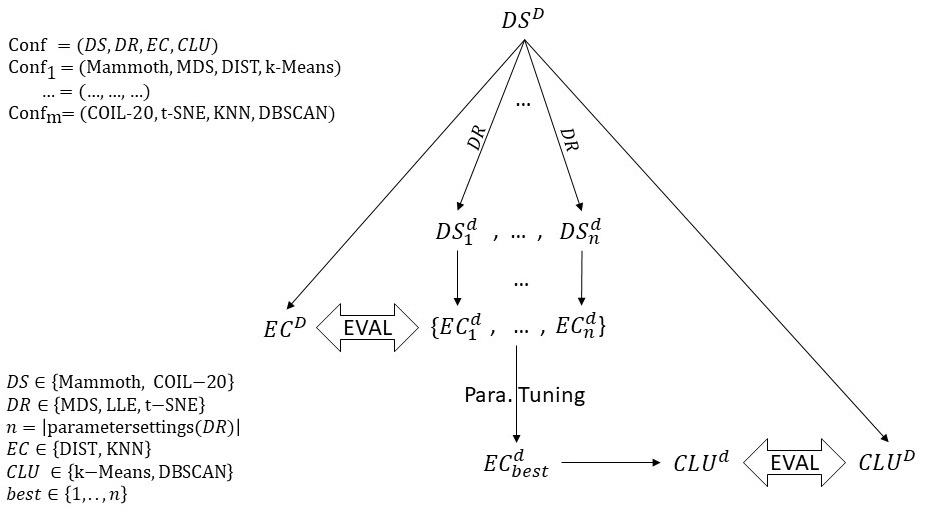
\includegraphics[width=1\columnwidth]{images/pipeline_final.jpg}
	\caption[Experimental Pipeline]{Pipeline of the experiments. Inputs are configurations defined in the top left corner. The variables and sets are defined in the bottom left corner.}
    \label{fig:pipeline}
\end{figure}

\section{Tools and System Specifications} \label{sec:toolsandsysspec}

To conduct the various experiments needed to evaluate the performance of the manifold learning methods we chose to use an offer from the University Computing Centre (HPC) called "caucluster"\footnotemark. This computing system provides powerful resources for scientific computing and it has the following system specifications:
\footnotetext{\url{https://www.rz.uni-kiel.de/en/our-portfolio/hiperf/caucluster}}
The cluster consists of 2 login nodes with a GPU and 130 compute nodes without one. On every node the CPU \textit{AMD Epyc 7313 (Milan)} with 32 cores running at 3.0GHz is installed, resulting in a total capacity of 4160 cores. Furthermore, every node has at least 256GB and up to 4096GB of main memory.

On these machines \textit{slurm} (Simple Linux Utility for Resource Management) is installed which enabled us to efficiently and automatically distribute and parallelize our calculations across all available compute nodes. As a foundation, we set up a \textit{python} (v3.10) \textit{virtual environment} with our desired libraries. The most important library is the \textit{scikit-learn} (v1.3) as it provides the implementation of the manifold learning methods we will compare in this work. Beyond that, they also provide the needed clustering algorithms and some important evaluation measures. The second important library we used is \textit{matplotlib} (v3.7). This was used to plot our datasets as well as the low dimensional embeddings and the graphs resulting from the evaluations. In our case, we have made special use of heatmaps, scatter-, and line-plots. Another useful library was \textit{NumPy} (v1.25) with its very optimized and powerful mathematical operations especially for matrices. Further, two libraries namely \textit{pillow} (v10.0) and \textit{pandas} (v2.1) were used which just had a small use case. Pillow for opening images and pandas for sorting and printing evaluation results.

\section{Acquisition of Evaluation Data} \label{sec:acq_data}

Here we will go into detail about the acquisition of our evaluation data. We noticed that we had a lot of data that had to be calculated. The types of data are the following: the most important ones are the low dimensional embeddings of the datasets derived from the application of LLE and t-SNE. Additionally, we calculated for all parameter settings of those methods our distance and neighborhood evaluation measure. After that, we calculated the clusterings for some embeddings for all clustering parameter settings with the corresponding clustering evaluation measures. For the MDS method, we just had to calculate a single run for all the types of data we needed as the method has no parameter settings.
As we have mentioned in Section \ref{sec:toolsandsysspec}, we made use of slurm on the caucluster. On this system, every user has a maximum limit of simultaneous usage of 1024 CPU cores and 16TB of main memory. With this limitation, we have made use of 1000 cores and 15.5TB memory simultaneously by assigning a slurm array job with one core and 15.5GB memory per job. The resulting fragmented data was then merged into a single file.
The most expensive calculations were the calculations of the low dimensional embeddings. To illustrate the enormous time complexity of the LLE method we have made the Figures \ref{fig:drONmamm} and \ref{fig:drONcoil}. By visually inspecting the two graphs we see a hint towards a constant pattern on t-SNE calculations and an exponential pattern on LLE calculations. This shows us that LLE's time complexity is very high.
For the reason that we could run 1000 jobs at the same time the deployment of LLE on the Mammoth dataset had a total execution time of 139h (5.8d) compared to 1.53h (0.06d) for t-SNE on Mammoth.
\begin{figure}[!]
	\centering
	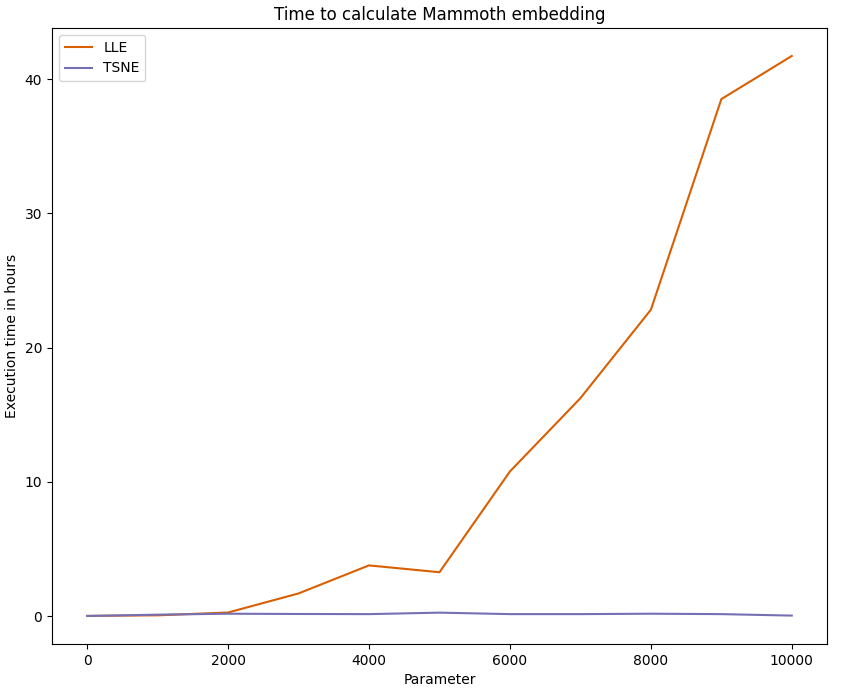
\includegraphics[width=0.80\columnwidth]{images/drONmamm.png}
	\caption[DR on 3D-Mammoth]{The execution times of deploying the manifold learning methods on the 3D-Mammoth dataset. The results are analogous to the transformed Mammoth dataset. Total execution time, \textcolor{lle}{LLE: 139h}, \textcolor{tsne}{t-SNE: 1.53h}.}
    \label{fig:drONmamm}
\end{figure}
\begin{figure}[!]
	\centering
	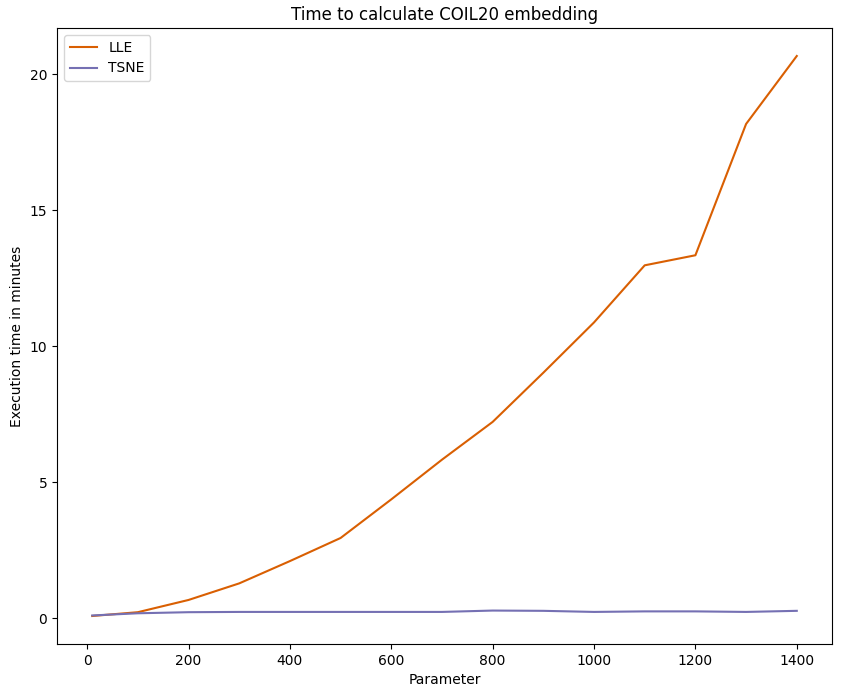
\includegraphics[width=0.80\columnwidth]{images/drONcoil.png}
	\caption[DR on COÌL-20]{The execution times of deploying the manifold learning methods on the COIL-20 dataset. Total execution time, \textcolor{lle}{LLE: 1.83h}, \textcolor{tsne}{t-SNE: 0.06h}.}
    \label{fig:drONcoil}
\end{figure}